% Template created by Joseph Petitti in 2018
% Released under the CC0 Universal Public Domain Dedication license
% https://creativecommons.org/publicdomain/zero/1.0/
% You can do whatever you want with this, you don't even have to cite me

\documentclass[a4paper, 12pt, american]{article}

% useful packages
\usepackage[utf8]{inputenc}
\usepackage[american]{babel}
\usepackage{csquotes}
\usepackage[margin=1in]{geometry}
\usepackage{lipsum}
\usepackage{graphicx}
\usepackage{setspace}
\usepackage[page, titletoc, title]{appendix}
\usepackage[
    style=apa,
    backend=biber,
    sortcites=true,
    sorting=nyt,
%    isbn=false,
%    url=false,
%    doi=false,
%    eprint=false,
    hyperref=false,
    backref=false,
%    firstinits=false,
]{biblatex}

% declare useful stuff for LaTeX to know
\DeclareLanguageMapping{american}{american-apa}
\graphicspath{ {./images/} } % this is where you'll put all your images
\bibliography{references}
\title{Put Your Title Here}
\author{Put your names here}
\date{\today}

\begin{document}
% set page numbers to Roman for the forematter (before the introduction
\pagenumbering{roman}

% Title page
\begin{center}
{\huge Put Your Title Here}
\vfill
An Interactive Qualifying Project \\
Submitted to the Faculty of \\
WORCESTER POLYTECHNIC INSTITUTE \\
in partial fulfilment of the requirements for the \\
Degree of Bachelor of Science\par
\vfill
by \\
Group Member 1 \\
Group Member 2 \\
Group Member 3 \\
Group Member 4\par
\vfill
Date: \\
\today\par
\vfill
Report Submitted To:\par
\end{center}
\vspace{\baselineskip}
\begin{flushright} % list your sponsors and 
	Sponsor 1 \\
	Sponsor Organization 1 \\
	\vspace{\baselineskip}
	Sponsor 2 \\
	Sponsor Organization 2\par
	\vspace{\baselineskip}
	Professors Adviser 1 and Advieor 2 \\
	Worcester Polytechnic Institute
\end{flushright}
\vfill
\newpage

\onehalfspacing % the meat of your report will be 1.5 spaced
\begin{abstract}
	This is where your abstract should go.
	\lipsum[3]
\end{abstract}
\newpage

\section*{Acknowledgements}
\addcontentsline{toc}{section}{Acknowledgements}

\lipsum[3]

\newpage

\section*{Executive Summary}
\addcontentsline{toc}{section}{Executive Summary}

\lipsum[3]

\newpage

\section*{Authorship}
\addcontentsline{toc}{section}{Authorship}

\lipsum[3]

\newpage
\singlespacing % make the table of contents, figures, and tables single spaced

\tableofcontents

\listoffigures

\listoftables

\newpage
\onehalfspacing % revert back to 1.5 spacing
\pagenumbering{arabic} % switch to Arabic numbering for the main part
\section{Introduction}

\lipsum[8]

\newpage

\section{Background}

\subsection{This is a subsection}

In this section, we introduce something blah blah blah.

\subsubsection{This is a subsubsection}

By definition from Merriam-Webster, culture refers to ``the characteristic
features of everyday existence shared by people in a place or time.'' Here's
a random fact to show you how citations work. Cantopop flourished in Hong Kong
in the 1970s, as a genre of love songs with Cantonese lyrics backed by western-
style pop music \parencite{carroll2007}.

\lipsum[1]

\subsubsection{Here's another subsubsection}

\lipsum[3]

% this is a picture with a caption
\begin{figure}[h]
	\centering
	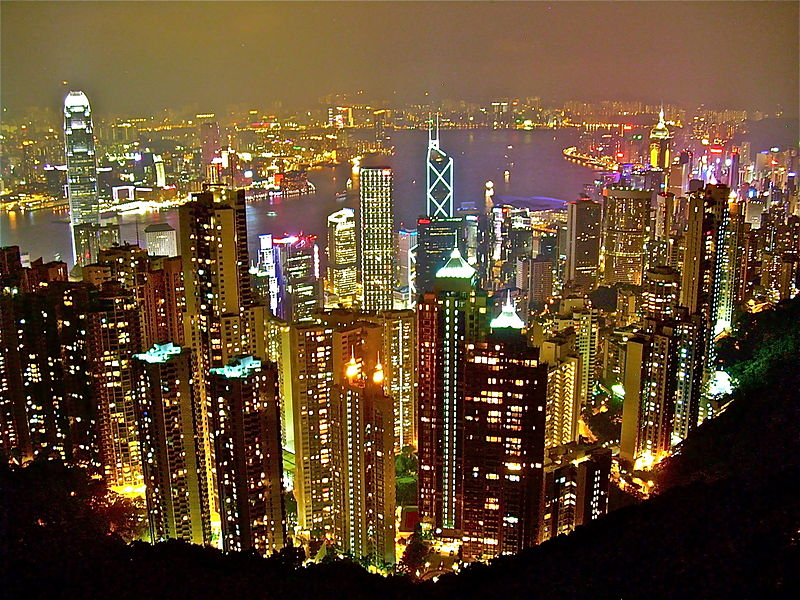
\includegraphics[width=\textwidth]{hong-kong-skyline.jpg}
	\caption{Hong Kong skyline as seen from Victoria Peak, 2009 (CC0 1.0)}
\end{figure}

\subsection{Here's a new subsection}

\lipsum[1]

\subsubsection{And a new subsection}

\lipsum[4]

\subsubsection{You probably get the point now}

\lipsum[1]

\newpage

\section{Methodology}

\lipsum[1]

\newpage

\section{Findings}

\lipsum[1]

\newpage

\section{Conclusions \& Recommendations}

\lipsum[1]

\newpage

\section*{References}
\addcontentsline{toc}{section}{References}

\printbibliography[heading=none]

\newpage

\appendices

\section{This is your first appendix}

You can add other appendices with sections the same way.

\lipsum[4]

\end{document}
